\chapter{Non-local similarity-based propagation model} 
\label{chap_NLM} 

This chapter proposes a novel model that combines low-resolution measurements in space and time in order to reconstruct fully resolved turbulent fields. This method tackles the problem of fusing high-time-low-space and low-time-high-space resolution measurements mentioned in section \ref{sec:probdef2}. The model exploits local structures in large scale measurements to reconstruct small scales. The idea is to assume that small scales are essentially advected by large scales. This is based on the scale similarity hypothesis, where information at adjacent ranges of scales are strongly correlated. The model is further developed from the non-local means (NLM) denoising filter \citep{buades2005review}, which is very simple but efficient, and widely used in image processing.

The proposed model is applied to the streamwise velocity fields from DNS data of isotropic turbulence as described in section \ref{sec:data_isotropic}. Due to the absence of time resolved fields, \textit{the streamwise direction is associated to the time dimension}, while the other two spatial directions are the spanwise and the vertical ones. Within this chapter, parameters of the model will be optimized. Model performances are also investigated by fixing one subsampling ratio in either space or time (spanwise) while varying the other. Detailed analysis of model performances are presented, but further comparisons with other methods will be investigated in chapter \ref{chap_comparisons}.

\section{Non-local means}
Non-local means (NLM) was originally proposed by \citet{buades2005review} to deal with the single image denoising problem. It has been then extended to solve other inverse problems of image reconstruction such as inpainting (to fill in missing pixels) or super-resolution (to increase image resolution). The model assumes that image content is likely to repeat in many regions. The estimate of each pixel is a weighted average of its neighbors assigned with different weights. These weights are estimated as the similarity of the denoised/inpainted/super-resolved pixel with its neighbors. By proposing several estimates of a single pixel, NLM yields redundancy by using several observations of similar scenes obtained from different locations within the same image. These multiple observations of underlying ground truth help in solving the ill-posed inverse problem.

\subsection{Non-local means filter for denoising}
\begin{figure}
	\centering
	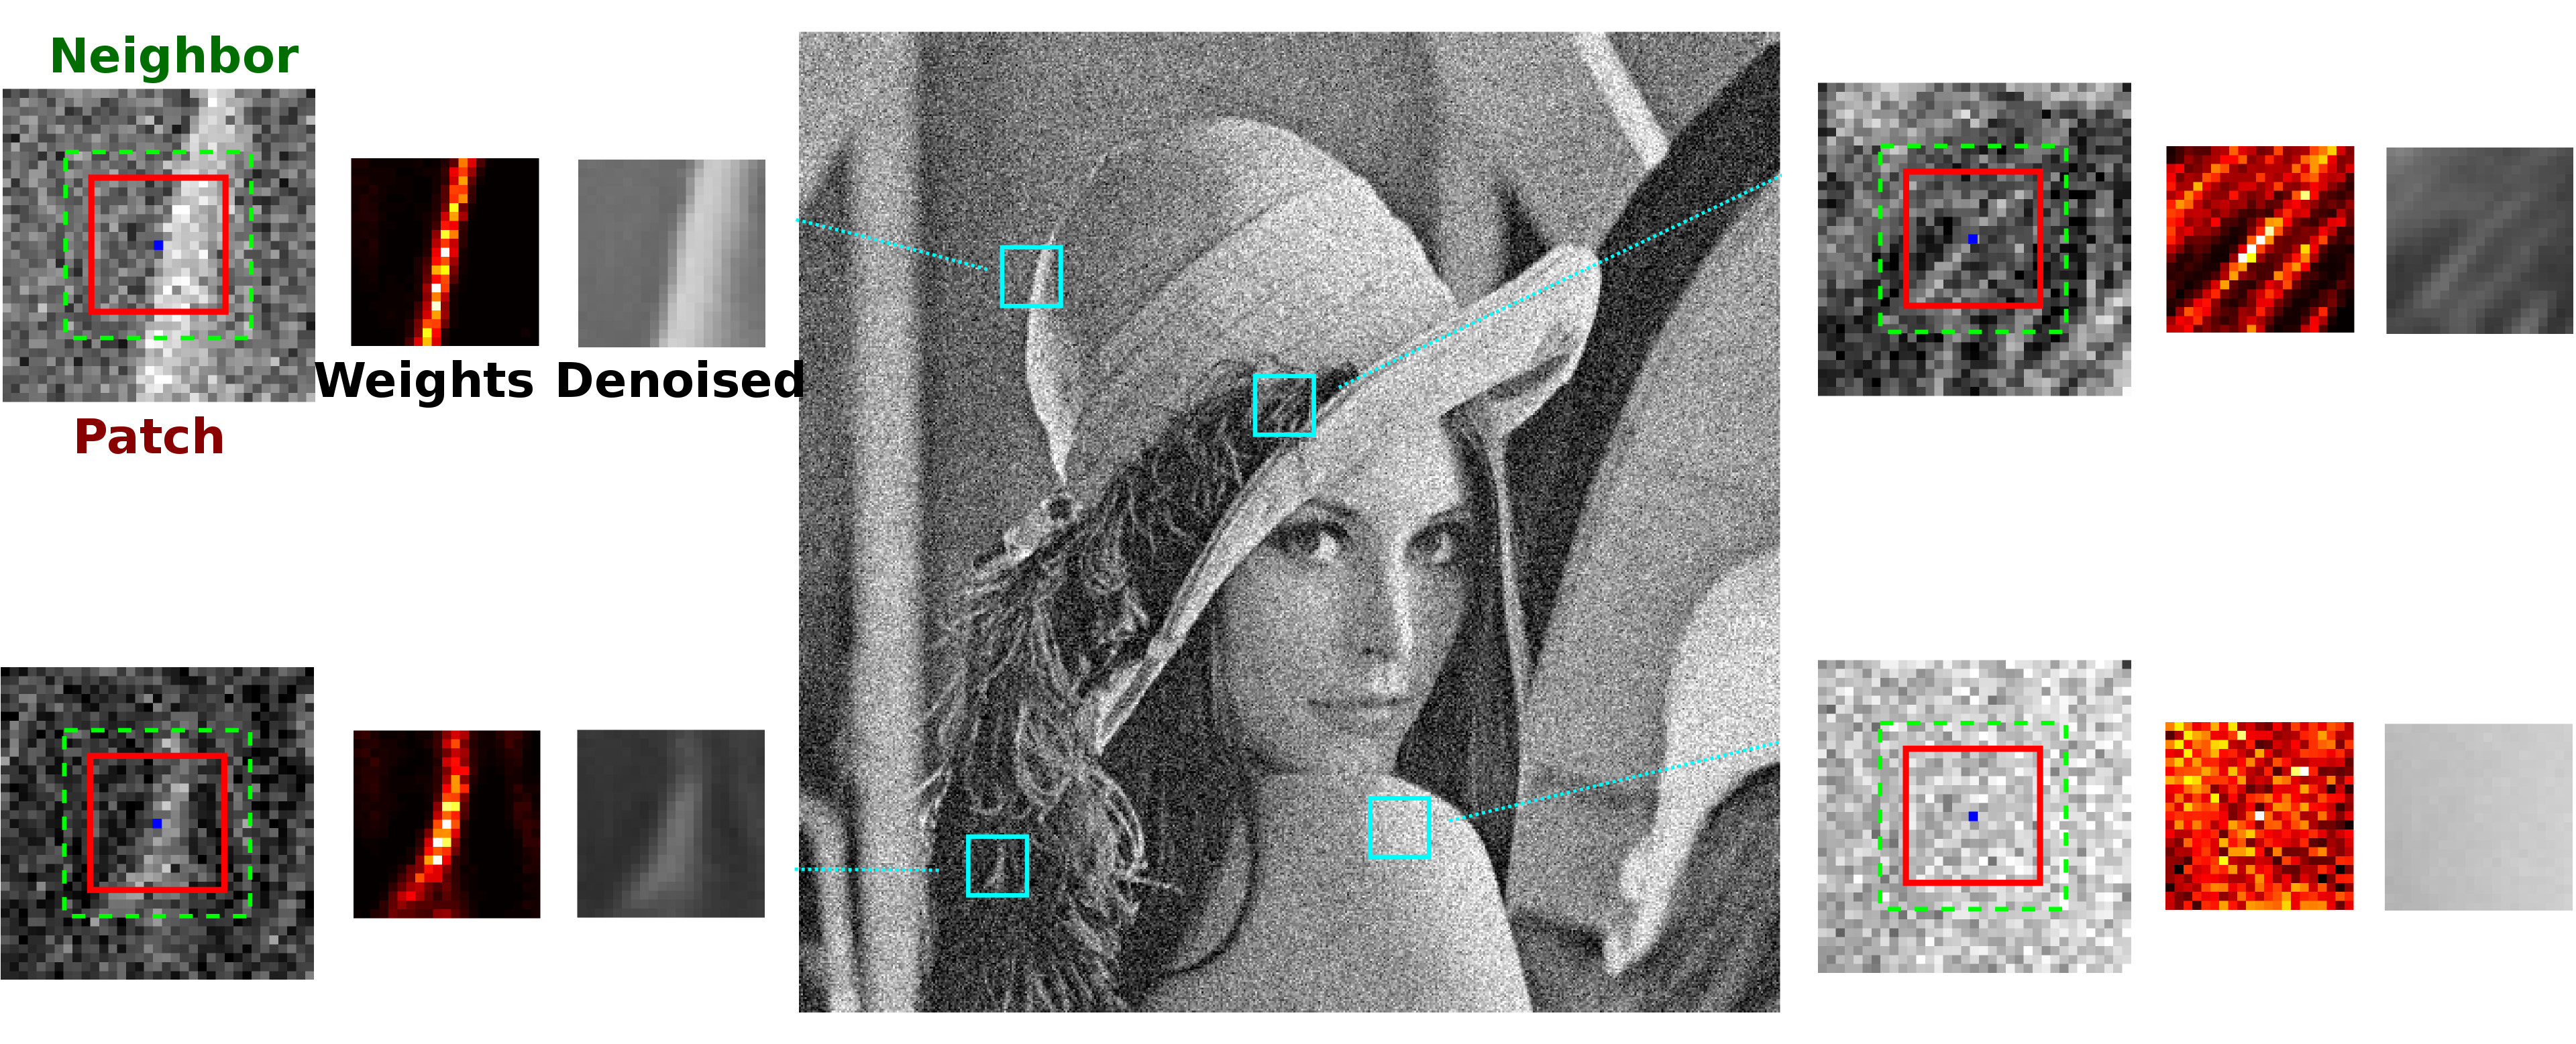
\includegraphics[width=\columnwidth]{./images/NLM/lena.png}		
	\caption{\label{fig:lena} Image denoising using non-local means. Four sample patches in red extracted from noisy image and centered at blue dots. The estimate of each point are weighted average of its neighbors, and weights are computed as the similarity of the moving patches compared to the reference patch. Photo credit: \citet{foi2016foveated}.}
\end{figure}

The NLM denoising filter is simple but rather robust. Figure \ref{fig:lena} illustrates how the NLM filter works on a sample image. Denoting $ \mybold{z}_t \in \R^{\dimsh} $ as the column vector of a 2D noisy image, the NLM filter denoises the $ k- $th pixel as a weighted average of its neighboring noisy pixels:
\begin{equation}
	\hat{\mybold{z}}_t[k]=\frac{\displaystyle \sum_{i\in\neighbor_k}w[k,i]\mybold{z}_t[i]}{\displaystyle \sum_{i\in\neighbor_k}w[k,i]}
\end{equation}
$ \neighbor_k $ is the set of neighboring pixels of the $ k- $th pixel. The local weight coefficient $ w[k,i] $ is the similarity between the $ k- $th and $ i- $th pixels:
\begin{equation}
	w[k,i] = \myexp{ -\frac{\|\mathcal{R}_s^k\mybold{z}_t-\mathcal{R}_s^i\mybold{z}_t\|^2_2}{2\nlmfilparam^2}}
\end{equation}
where the operator $ \mathcal{R}_s^k: \R^{\dimsh} \mymapto \R^\dimpsh$ extracts 2D patches of size $ \sqrt{\dimpsh}\times \sqrt{\dimpsh} $ centered at the $ k- $th pixel. These patches are then arranged in a column vector in lexicographical order. When $ \dimpsh=1 $, the NLM filter becomes a bilateral one. The global filter parameter $ \sigma $ regulates the decay of the exponential expression. It controls the contribution of the $ i- $th pixel on the estimation of the $ k- $th pixel. Geometrical priority can also be introduced, where high weights are given to closer neighbors than further ones.


\subsection{Generalized non-local means for super-resolution}
The idea of the NLM filter has been generalized to perform video super-resolution \citep{protter2009generalizing} by introducing time dimension. The aim is to estimate HR sequence of images $ \mybold{z}_t \in \R^{\dimsh}, t=1,2,...,\dimth , $ from corresponding LR sequence of images $ \mybold{y}_t \in \R^{\dimsl}$ ($ \dimsl <\dimsh $). NLM exploits the self-similarity property of natural images in the sequence. The model assumes that common scenes are shared by many snapshots in the sequence. Derivation and mathematical explanation can be found in \citet{protter2009generalizing}. The closed form solution is simplified, where each HR pixel is estimated as a weighted average of neighboring LR pixel in a space-time window:
\begin{equation}
	\hat{\mybold{z}}_{t_\knot}[k]=\cfrac{\displaystyle \sum_{t\in\neighbor_{t_\knot}}\sum_{i\in\neighbor_k}w[k,i,t]\mybold{y}_t[i]}{\displaystyle \sum_{t\in\neighbor_{t_\knot}}\sum_{i\in\neighbor_k}w[k,i,t]}
\end{equation}
where $ \neighbor_{t_\knot} $ is the set of neighboring snapshots in time of the $ t_\knot$-th one. The weight $ w[k,i,t] $, defined as the probability of the $ k- $th HR pixel estimation coming from the $ i $-th LR pixel, is estimated as:
\begin{equation}
	w[k,i,t] = \myexp{ -\frac{\normtwo{\mathcal{R}_s^k\mybold{y}_{t_\knot}-\mathcal{R}_s^i\mybold{y}_t}}{2\nlmfilparam^2}}
\end{equation}
This solution exits when there is at least one non-zero weight $ w[k,i,t] $.

It is natural to test this idea to reconstruct HTHS turbulent fields $ \Z $ of size $ \dimth \times \dimsh $ from the corresponding HTLS measurements $ \Y $ of size $ \dimth \times \dimsl $ ($ \dimsl < \dimsh $) subsampled directly from $ \Z $. However, the NLM model by \citet{protter2009generalizing} is not able to improve the reconstruction accuracy compared to the single interpolation of HTLS velocity fields. This is potentially due to the differences between video of natural images and turbulence. The generalized NLM was originally illustrated most successful for video of human with small motions, where the same scene is obtained for successive snapshots. Turbulent fields are fundamentally different, where no sharp edge exists, sizes of structures make a continuous spectrum, and all scales move and distort randomly. Also, since turbulence fields have a decreasing power law spectrum, large scales contain most of the kinetic energy. The reconstruction of these information plays the dominant role in total error. The current NLM model re-estimates large scales, which are probably not as good as by spline interpolation. 

\section{Similarity-based model to propagate small scales}
\begin{figure}
\centering
	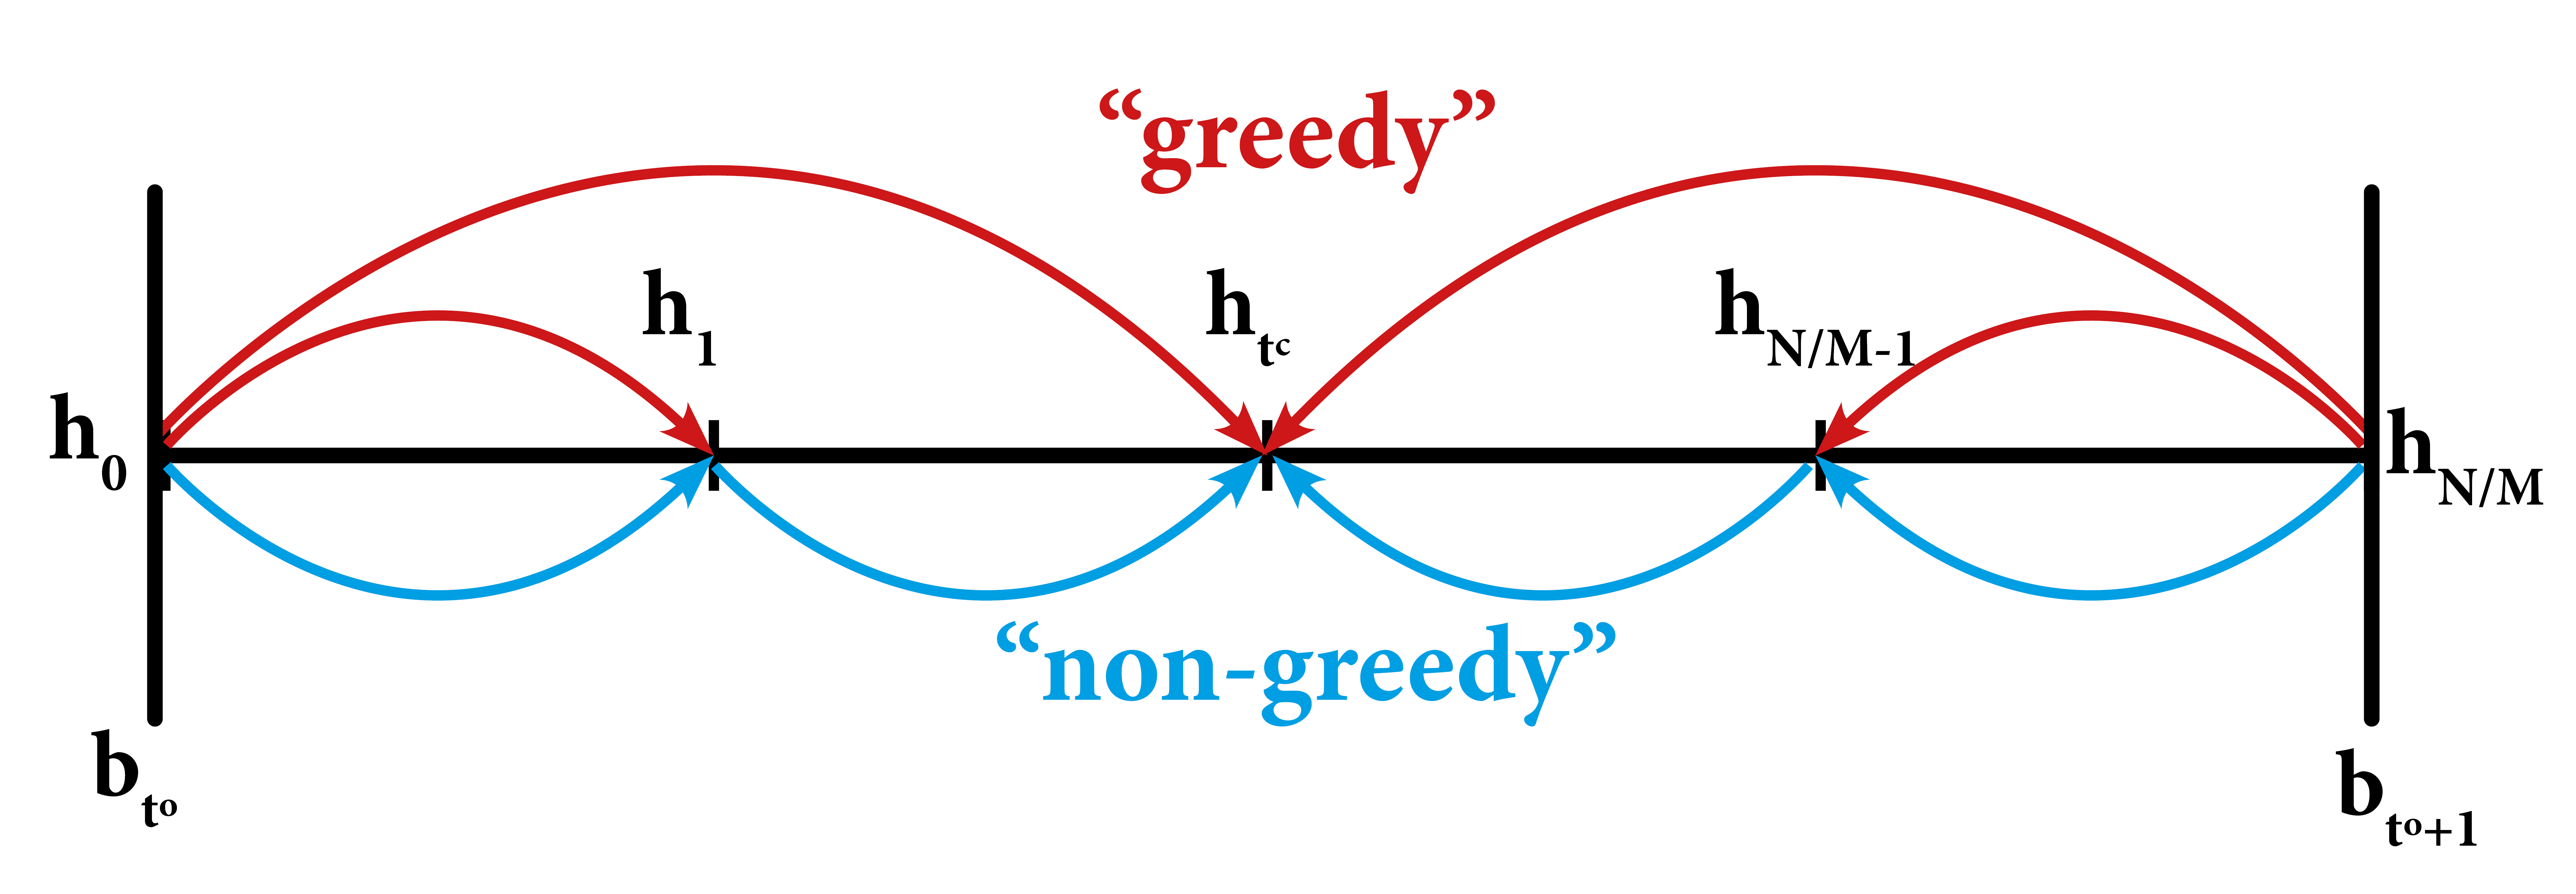
\includegraphics[width=0.8\columnwidth]{./images/NLM/propagation_scheme.png}
	\caption{\label{fig:propagation_scheme} A sketch of \textit{greedy} and \textit{non-greedy} propagation models. The two LTHS planes are at the border including small scales $ \boundHF_{t_\knot} = \h_0 $ and $ \boundHF_{t_\knot+1} = \h_{\dimth/\dimtl} $ defined in equation \ref{eq:greddy1}. All small scales to be estimated from other planes $ \h_1, \h_2,...,\h_{\dimsh/\dimsl-1} $ will be propagated either directly from LTHS planes (greedy, red arrows) or in a plane-by-plane manner (non-greedy, blue arrows). To simplify the plot, the propagation is shown from LTHS planes till the central plane only.}
\end{figure}

We propose a similarity-based model in the spirit of the NLM model for video super-resolution with important modifications. Since large scales are well reconstructed also with spline interpolation, we leave these information unchanged while propagating small scales only. Two models, the so-call ``\textit{greedy}'' and ``\textit{non-greedy}'' propagations, are proposed. Figure \ref{fig:propagation_scheme} illustrates the idea of the two propagation schemes. While the greedy model propagates small scales from LTHS planes directly toward other instant, the non-greedy one does the propagation plane-by-plane.

\subsection{Greedy propagation of small scales from key planes}
LTHS measured snapshots are crucial to recover some spatial HF contents, since these are the only place where small scales are available. In the configuration presented in figure \ref{fig:space-time_measurements}, HTLS snapshots give only information of large scales in space, while small ones are only accessible from LTHS snapshots. The idea is to bring these small-scale information and aggregate them on top of the measured large scales. The propagation model is based on the similarity of large scales at different instants, while assuming that small scales are advected by large ones.

LTHS snapshots $ \{\x_{t_\knot} \} \in \R^{\dimsh}, t_\knot = 1,2,...,\dimtl$, also called \textit{key frames}, include both large and small scales. HTLS snapshots $ \{\y_t \}  \in \R^{\dimsh}, t=1,2,...,\dimth$ contain only large scales. The propagation model aims at propagating the small-scale content from the key frames and aggregating with the interpolation $ \Interp_s\y_t $ to reconstruct $  \myhat{\z}_t $, which contains information of all scales. $ \Interp_s: \R^{\dimsl} \mymapto \R^{\dimsh} $ is the 2D cubic spline interpolator to reconstruct large scales from LR measurements. 

The propagation is based on the similarity of the large scales between the key frames and the measured planes to reconstruct. Large and small scales could be separated from the key frames using ideal Fourier filter. However, these large scales are not consistent with those from the measured planes obtained by interpolations. It is more consistent to subsample and re-interpolate LTHS fields the same way as HTLS ones. Small scales of each key frame are then defined as:
\begin{equation}
\boundHF_{t_\knot} = \mybold{x}_{t_\knot} - \Interp_s\Sub_s\mybold{x}_{t_\knot}
\label{eq:greddy1}
\end{equation}
$ \Sub_s $ is the subsampling operator in space, $ \Sub_s: \R^{\dimsh} \mymapto \R^{\dimsl} $, and $ \boundHF_{t_\knot} $ should contain some aliasing. The greedy propagation model estimates small scales $ \h_t $ at the $ t- $th time step from the given small scales  $ \boundHF_{t_\knot} $ and $ \boundHF_{t_\knot+1} $ of the two bounded LTHS planes, ones just before and after the $ t $-th HTLS plane in time:
\begin{equation}
	\hat{\h}_t[k]=\cfrac{\displaystyle \sum_{i\in\neighbor_k}w_0[k,i,t]\boundHF_{t_\knot}[i] + \sum_{i\in\neighbor_k}w_1[k,i,t]\boundHF_{t_\knot+1}[i]}{\displaystyle\sum_{i\in\neighbor_k}w_0[k,i,t] + \sum_{i\in\neighbor_k}w_1[k,i,t]}
\label{eq:greddy2}
\end{equation}
The weight $ w_0[k,i,t] $ measures the similarity of $ k-th $ pixel of $ \hat{\h}_t $ and the $ i $-th pixel of $ \boundHF_{t_\knot} $, and analogously for $ w_1[k,i,t] $. It is estimated as the similarity of large scales in the two snapshots:
\begin{equation}
w_0[k,i,t] = \myexp{ -\frac{\|\mathcal{R}_s^k\Interp_s\mybold{y}_t-\mathcal{R}_s^i\Interp_s\Sub_s\mybold{x}_{t_\knot} \|^2_2}{2\nlmfilparam^2}}
\label{eq:greddy3}
\end{equation}
The term $ \Interp_s\Sub_s\mybold{x}_{t_\knot} $ is the conjugate large scales of $ \boundHF_{t_\knot} $, i.e. $ \mybold{x}_{t_\knot} = \Interp_s\Sub_s\mybold{x}_{t_\knot} + \boundHF_{t_\knot} $. $ w_1[k,i,t] $ is estimated analogously. The final reconstruction of all scales is:
\begin{equation}
\myhat{\z}_t = \Interp_s \y_t + \myhat{\h}_t
\label{eq:greddy4}
\end{equation} 
Since $ \Interp_s \y_t $ contains some aliasing, so does $ \myhat{\h}_t $ due to the presence of aliasing in $ \boundHF_{t_\knot} $ and $ \boundHF_{t_\knot+1} $, we could hope the two aliasing terms cancel and make the estimate of $ \myhat{\z}_t $ more accurate. This can explain also the benefit when considering $ \boundHF_{t_\knot} $ as the residual of the interpolation instead of ideal small scales. 

The propagation in the formulation \ref{eq:greddy2} is point-wise, where each point is estimated as a weighted average of its neighbors. Instead, a small patch centered at $ i- $th pixel of $ \boundHF_{t_\knot} $ and $ \boundHF_{t_\knot+1} $ can be accumulated over the patch centered at the $ k- $th pixel of $ \hat{\h}_t $ using the same weights $ w_0[k,i,t] $ and $ w_1[k,i,t] $. Since the same pixel belongs to several patches, the overlapping as in the patch-based approach (section \ref{subsec:patch_based_estimation}) is used. The overlapping will ensure the continuity of neighboring points and increase the consistence of all existing structures. There will be also more degree of freedom, where the number of estimates at each location increases significantly. The accumulation of scales and weights are as:
\begin{equation}
\begin{split}
\hat{\h}_t &= \sum_{k = 1}^{\dimsh} \left( \left(\mathcal{R}_a^k\right)^{\mytrans}\left(\sum_{i\in\neighbor_k}w_0[k,i,t]\mathcal{R}_a^i\boundHF_{t_\knot}[i] + \sum_{i\in\neighbor_k}w_1[k,i,t]\mathcal{R}_a^i\boundHF_{t_\knot+1}[i]\right) \right)\\
W_t &= \sum_{k = 1}^{\dimsh} \left(\left(\mathcal{R}_a^k\right)^{\mytrans}\mathcal{R}_a^k\mybold{1} \left(\sum_{i\in\neighbor_k}w_0[k,i,t] + \sum_{i\in\neighbor_k}w_1[k,i,t]\right) \right)
\end{split}
\label{eq:greddy5}
\end{equation}
where $ \mathcal{R}_a^k $ and $ \mathcal{R}_a^i $ extract a small patch of size $ \sqrt{\dimpacc} \times \sqrt{\dimpacc} $ centered at the $ k- $th and $ i- $th pixel respectively. The transpose operator $ \left(\mathcal{R}_a^k\right)^{\mytrans} $ is to put back this small patch into the large field, centered at $ k- $th pixel. $ \mybold{1} $ is the vector of size $ \dimsh \times 1 $ of ones. The term $ \left(\mathcal{R}_a^k\right)^{\mytrans}\mathcal{R}_a^k\mybold{1} $ puts ones at the position of each patch. The whole procedure is to accumulate the sum of all small scales estimates and their corresponding weights. The final step is the normalization:
\begin{equation}
\hat{\h}_t[k] \mymapfrom \cfrac{\hat{\h}_t[k]}{W_t[k]}
\label{eq:greddy6}
\end{equation}

\subsection{Non-greedy propagation of small scales}
The greedy model aims at propagating directly small scales from the two key frames to the HTLS planes. The performance of such a model is very limited when the similarity level decays rapidly with time far from the LTHS planes. A non-greedy propagation of small-scale information plane-by-plane from the two neighboring LTHS fields toward further planes is expected to improve the reconstruction. 

\begin{algorithm}[t]
\caption{Estimating small scales of $ \dimth/\dimtl - 1 $ planes by non-greedy NLM propagation from the two key frames at $ t_\knot $ and $ t_\knot+1 $} \label{algo_NLM_timepropagation}
\begin{algorithmic}[1]
	\State Input: $ \h_0 \mydef \boundHF_{t_\knot} $, $  \h_{\dimth/\dimtl} \mydef \boundHF_{t_\knot+1} $
	\State $ t_c = round(\dimth/2\dimtl) $ \Comment{Centered snapshot}
	\For {$ i = 1, ..., t_c-1$}
		\State $ j = \dimth/\dimtl - i$
		\State $ \h_i = g(i, \h_{i - 1},\h_{j + 1})$
		\State $ \h_j = g(j, \h_{i - 1},\h_{j + 1})$
	\EndFor
	
	\If{$ rem(\dimth/\dimtl - 1) == 0 $} \Comment{Check if even, there are 2 centered snapshots}
		\State $ \h_{t_c} = g(t_c, \h_s[t_c-1],\h_s[t_c+2])$
		\State $ \h_{t_c+1} = g(t_c+1, \h_s[t_c-1],\h_s[t_c+2])$		
	\Else
		\State $ \h_{t_c} = g(t_c, \h_{t_c-1},\h_{t_c+1})$ \Comment{Estimate centered snapshot}	
	\EndIf	
\end{algorithmic}
\end{algorithm}

The main step to propagate the small scales from the two key frames at $ \boundHF_{t_\knot} $ and $ \boundHF_{t_\knot+1} $ is presented in algorithm \ref{algo_NLM_timepropagation}. $ g(t,\h_1,\h_2) $ is denoted as the similarity-based estimation of small-scale information at $ t- $th plane from the two bounded planes, with scales to propagate being $ \h_1 $ and $ \h_2 $. The procedure starts by propagating small scales from these two frames to their first two neighboring planes, $ \h_1 $ and $ \h_{\dimth/\dimtl - 1} $ in algorithm \ref{algo_NLM_timepropagation}, following the formula \ref{eq:greddy5}. The next step considers these two estimated $ \h_1 $ and $ \h_{\dimth/\dimtl - 1} $ as the new key frames and propagate them further. This procedure is repeated till the central planes that are equally far from $ \boundHF_{t_\knot} $ and $ \boundHF_{t_\knot+1} $.

\section{Applying the propagation model to isotropic turbulence}
\subsection{The choice of model parameters}
The propagation model uses several parameters (see equations \ref{eq:greddy3} and \ref{eq:greddy5}), including the filter parameter $ \sigma $, the size $ \dimpsr $,  $ \dimpsh $, and $ \dimpacc $ of the searching region $ \mathcal{N}_s $, the similarity patch extracted by $ \mathcal{R}_s $, and the accumulation patch extracted by $ \mathcal{R}_a $ respectively. Optimization of these parameters is done by varying one while fixing the remaining three. The parameter-tunning is carried out by investigating the error between the reconstructed fields and the reference ones. These tests give an idea on the optimal set of parameters, which can be used in new situations where reference fields are not available. 

\begin{table} 
	\caption{\label{tab:NLMparams}
	Set of parameters to do simple grid search (try out all possible combinations from this set): the global filter parameter $ \sigma $, size of similarity patches $ \dimpsh $, size of accumulation patches $ \dimpacc $, and size of searching region $ \dimpsr $. The search is performed on the DNS data of isotropic turbulence, with the subsampling ratios are $ \dimsh/\dimsl = 3 \times 3 $ in space and $ \dimth/\dimtl = 4 $ in time.}
	\vspace{.5cm}
	\centering
	\begin{tabular}{S[table-format=1.2]S[table-format=2.0]S[table-format=2.0]S[table-format=2.0]} 
		\toprule
		{$\sigma$} & $\sqrt{\dimpsh}$ & {$\sqrt{\dimpacc}$} & {$\sqrt{\dimpsr}$}\\ 
		\midrule 
		0.05  &  9  & 1  & 5  \\ %\addlinespace
		0.1 & 17  & 3  & 11 \\ %\addlinespace
		0.2   & 25  & 13 & 17 \\ %\addlinespace
		0.4  &    & 25 &  \\ %\addlinespace
		\bottomrule
	\end{tabular}
\end{table}

Table \ref{tab:NLMparams} gathers all parameters to test. The DNS data of isotropic turbulence are used. HTLS and LTHS measurements are virtually extracted from the fully resolved fields as discussed in section \ref{sec:probdef2}. The subsampling ratios are $ \dimsh/\dimsl = 3 \times 3 $ in space, equally distributed in spanwise and vertical direction, and $ \dimth/\dimtl = 4 $ in time (streamwise). These subsamplings correspond to energy losses of about $ 1\% $ both in space and time (see table \ref{tab:energyloss_isotropic}). The configuration is chosen to have a moderate loss of information to facilitate all numerical experiments. Other configurations with various losses are investigated later in this section.

Three measures are used to study the effects of different parameters on the reconstruction accuracy. One is the average normalized root mean square error (NRMSE) $ \bar{\epsilon} $, which represents an overall measure of the reconstruction accuracy, as in equation \ref{eq:NRMSE}. The two other quantities are the power spectra $ E(k) $ and the spectra of the error $ E^{\epsilon}(k) $. Power spectra show streamwise energy contents, while error spectra show the squared errors at each frequency. These two measures give more insights about the model performances when reconstructing turbulent fields at different scales. 

\begin{figure}[t]
	\centering
	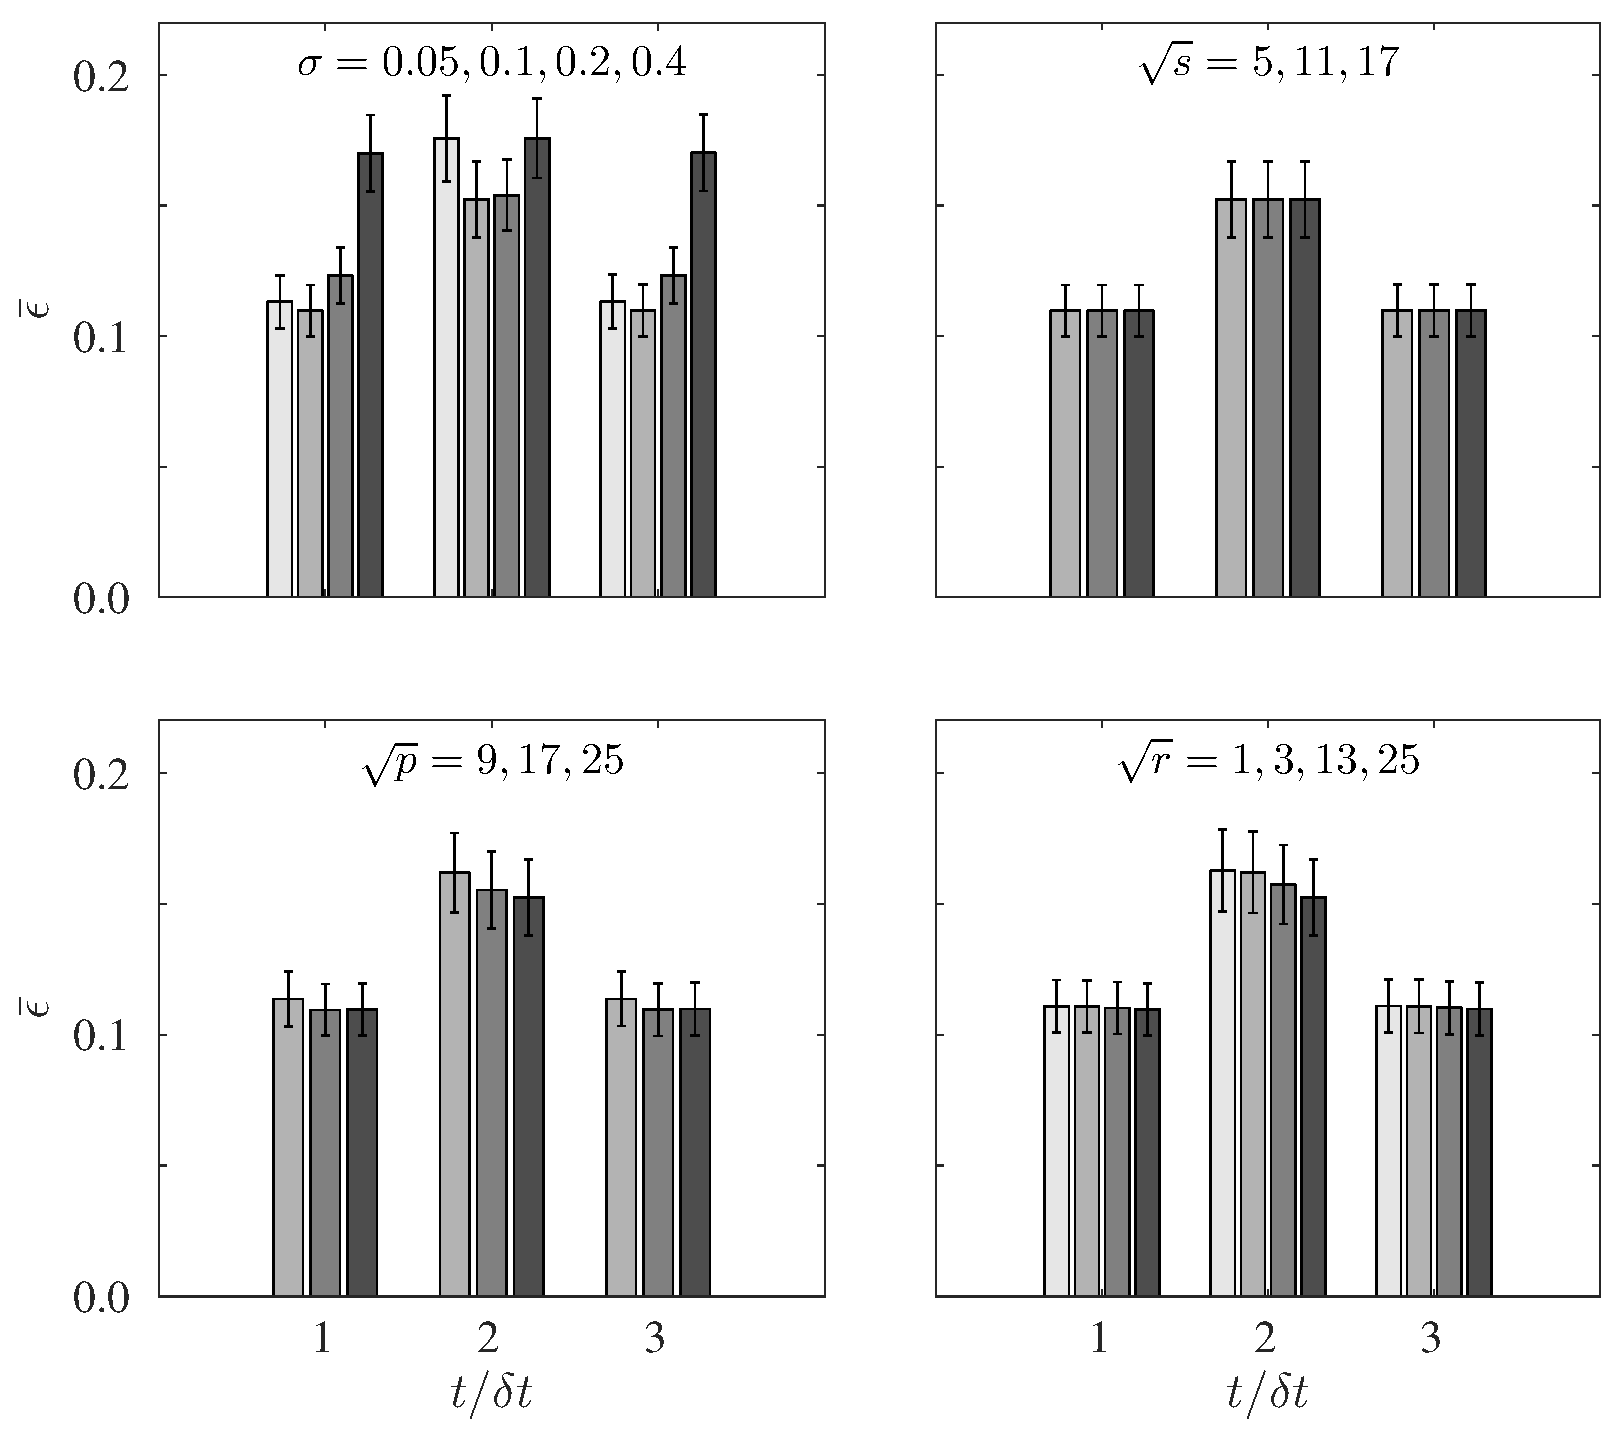
\includegraphics[width=\columnwidth]{./images/NLM/interpdiff/NLmean_propag1dir_spacing3_tspacing4_allparams_NRMSE.eps}
	\caption{\label{fig:NLM_various_params_NRMSE} Average NRMSEs over the whole dataset: each estimate of NRMSE is computed by comparing the reconstructed plane with the reference at each $ t/\delta t $. The bars show the average NRMSEs, while the error bars are standard deviations of NRMSE estimates.}
\end{figure}

Figure \ref{fig:NLM_various_params_NRMSE} shows average NRMSEs for different parameters as a function of $ t/\delta t $, the time distance from the previous LTHS plane to the estimated one. Two LTHS planes are at $ t/\delta t = 0 $ and $ t/\delta t = \dimth/\dimtl = 4 $. Average NRMSEs are shown as bars, with the standard deviation of each estimate shown by the error bars. The average and standard deviation of NRMSEs at each $ t/\delta t $ are computed using $ 37 \times 23 $ estimates from all blocks between the two successive key frames. Parameters are varied by changing one and keeping the remaining three constant around a reference parameters set ($ \sigma=0.1 $, $ \dimpsh=\dimpacc=25 \times 25 $ and $ \dimpsr = 11 \times 11$). This set is close to the optimal values used later in this section and chapter \ref{chap_comparisons} when comparing with other models.

\begin{figure}[t]
	\centering
	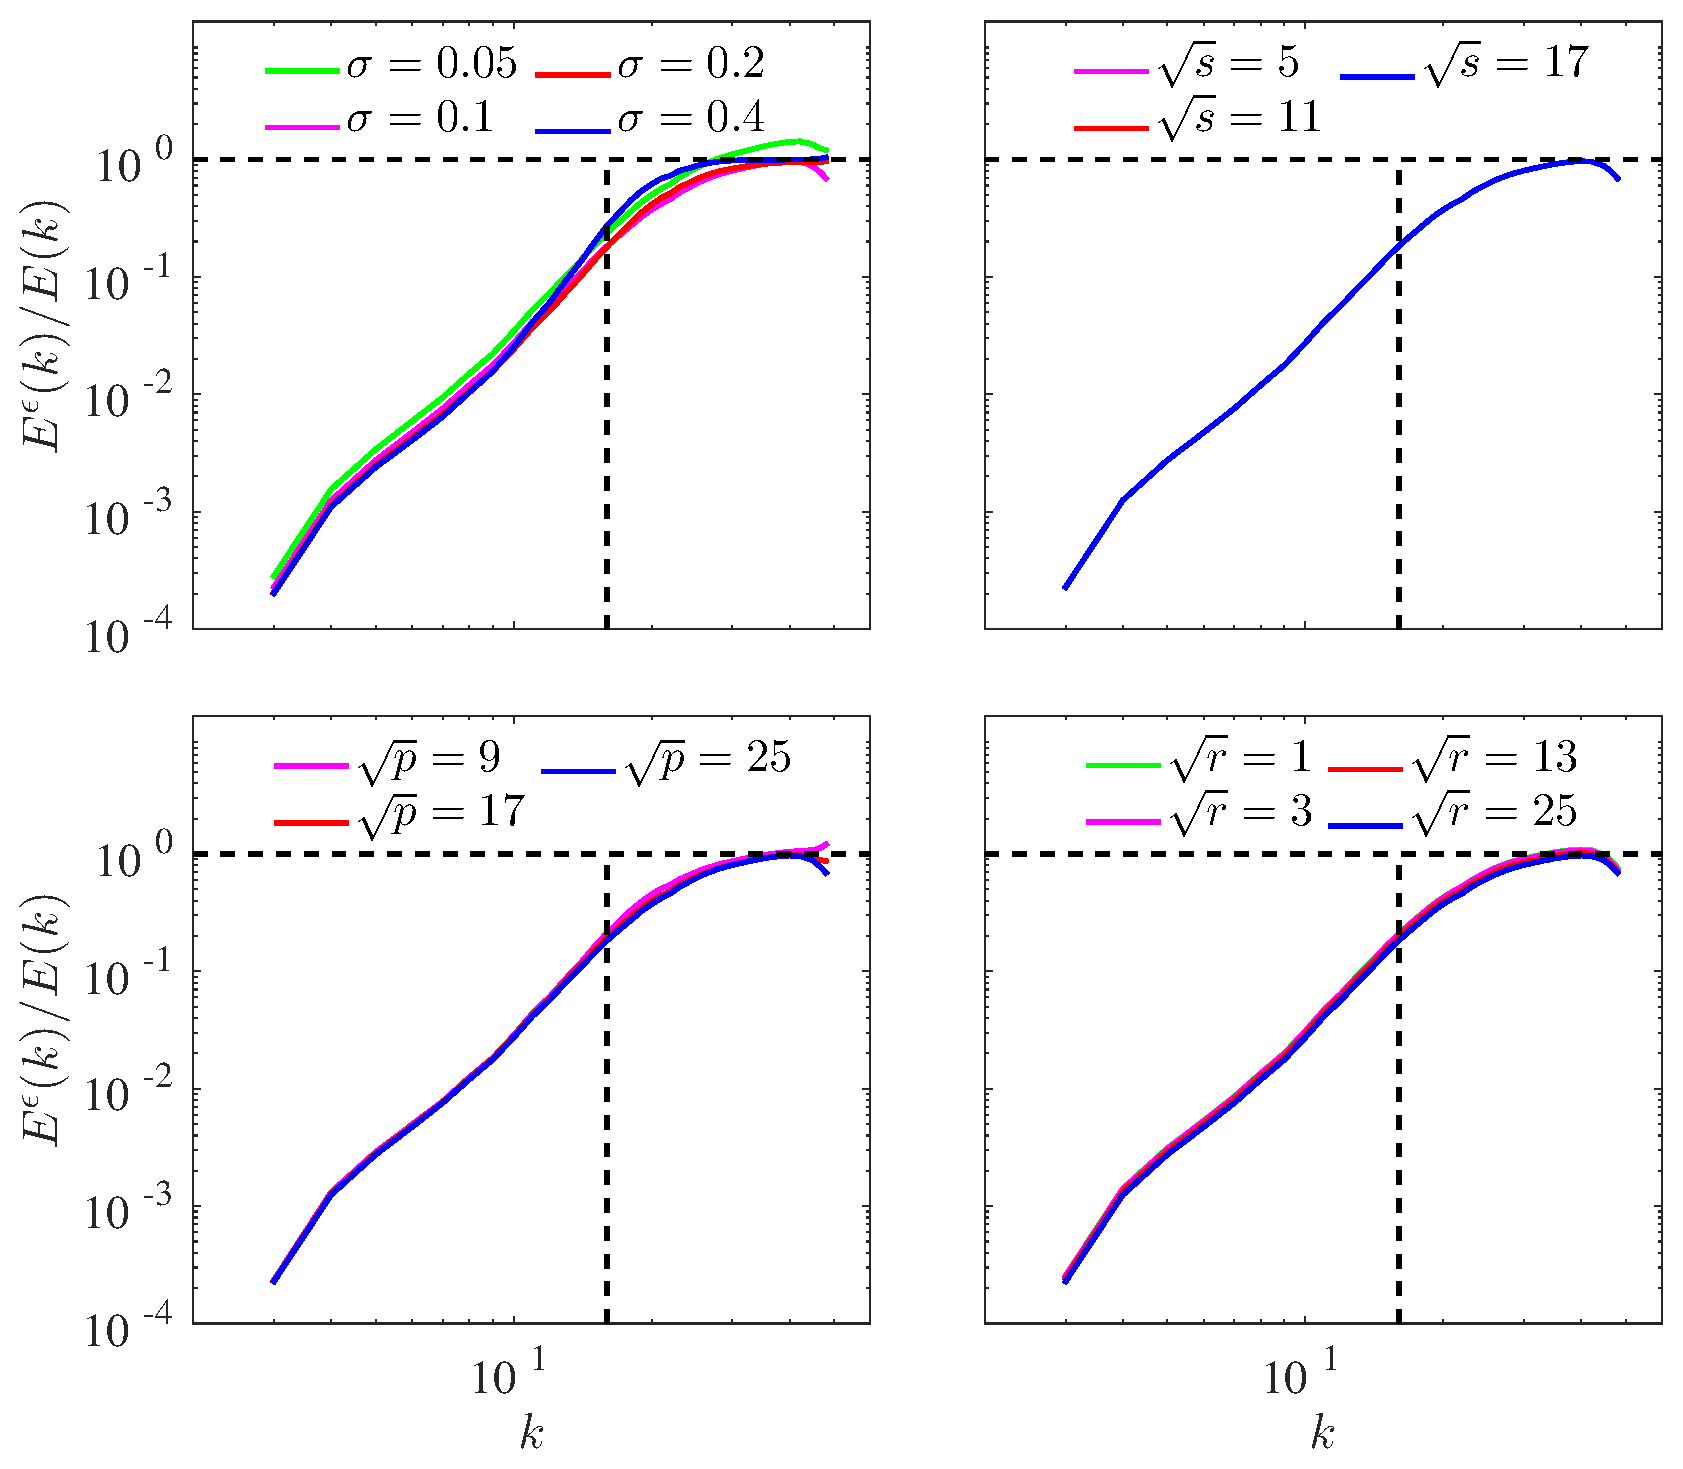
\includegraphics[width=\columnwidth]{./images/NLM/interpdiff/NLmean_propag1dir_spacing3_tspacing4_allparams_spectra.eps}
	\caption{\label{fig:NLM_various_params_spectra} Normalized error spectra of reconstructed planes at $ t/\delta t = 2 $ (the most remote from the two neighboring LTHS planes). Three cases of varying $ \dimpsh $, $\dimpacc$ and $\dimpsr$, all curves are almost collapsed.}
\end{figure}

Figure \ref{fig:NLM_various_params_spectra} shows the 2D spectra of the errors $ E^{\epsilon}(k) $ normalized by the energy spectra of the reference $ E(k) $. These spectra are estimated as an average of all planes at $ t/\delta t =2$, the most difficult planes to reconstruct. For all reconstructions, the spectra exhibit very small errors at large scales, which grow sharply when approaching the cutoff wave number defined by the spacing of the low sampling measurements. At very small scales, errors can reach $ 100 \% $. This level of error means that no information has been reconstructed. 

Among all parameters, the filter parameter $ \sigma $ is the most sensitive. The optimal value is $ \sigma \approx [ 0.1,0.2 ] $. Small values of $ \sigma $ narrow the searching region by shrinking weights of patches with low similarity levels to zero. Less estimates are taken into account when doing the weighted averaging. In the extreme situation $ \sigma = 0 $, the number of estimates is reduced to one pixel only, which is the center of the most correlated patch. The propagation model is simplified to the shifting of a single pixel. Otherwise, too large values of $ \sigma $ put weights on all the neighboring patches. Models with very large $ \sigma $ lead to a simple averaging with approximately equal weights. For these reasons, NRMSE is high for both small and large $ \sigma $, while a moderate value of $ \sigma $ is a good compromise to minimize the reconstruction error. This is shown in the error spectra (figure \ref{fig:NLM_various_params_spectra}) where the optimal $ \sigma $ gives similar large-scale reconstruction errors but lower ones at small scales.

Other model parameters are less sensitive. Searching region $ \mathcal{N}_k $ defines how large is the neighborhood to seek the small-scale information. However, the filter parameter $ \sigma $ plays a similar role by dumping the contribution of irrelevant patches to zero. Sizes of similarity and accumulation patches are more important. Similarity patches directly define the quality of weight estimates. Small patches are necessary to keep small-scale details of the flow. Larger patches improve the robustness of the models against noise and ill-posed conditions of the inverse problem. Ideally, we want the model to work well with small patches. However, experiments show slight improvements with larger patches. Similar results are observed when increasing the size of accumulation patches. Taking more pixels into the averaging helps in reducing the estimation noise, hence improving the reconstruction. 

\subsection{Comparing to spline interpolation}
The proposed propagation models, either greedy or non-greedy algorithm in time, are compared to cubic spline interpolations either in time $\Interp_t \mybold{x}_t $ or in space $\Interp_s \mybold{y}_t$. Apparently, $ \Interp_t \mybold{x}_t $ contains no temporal small-scales information, while $ \Interp_s \mybold{y}_t $ provides only large scales in space.

\begin{figure}
	\centering
	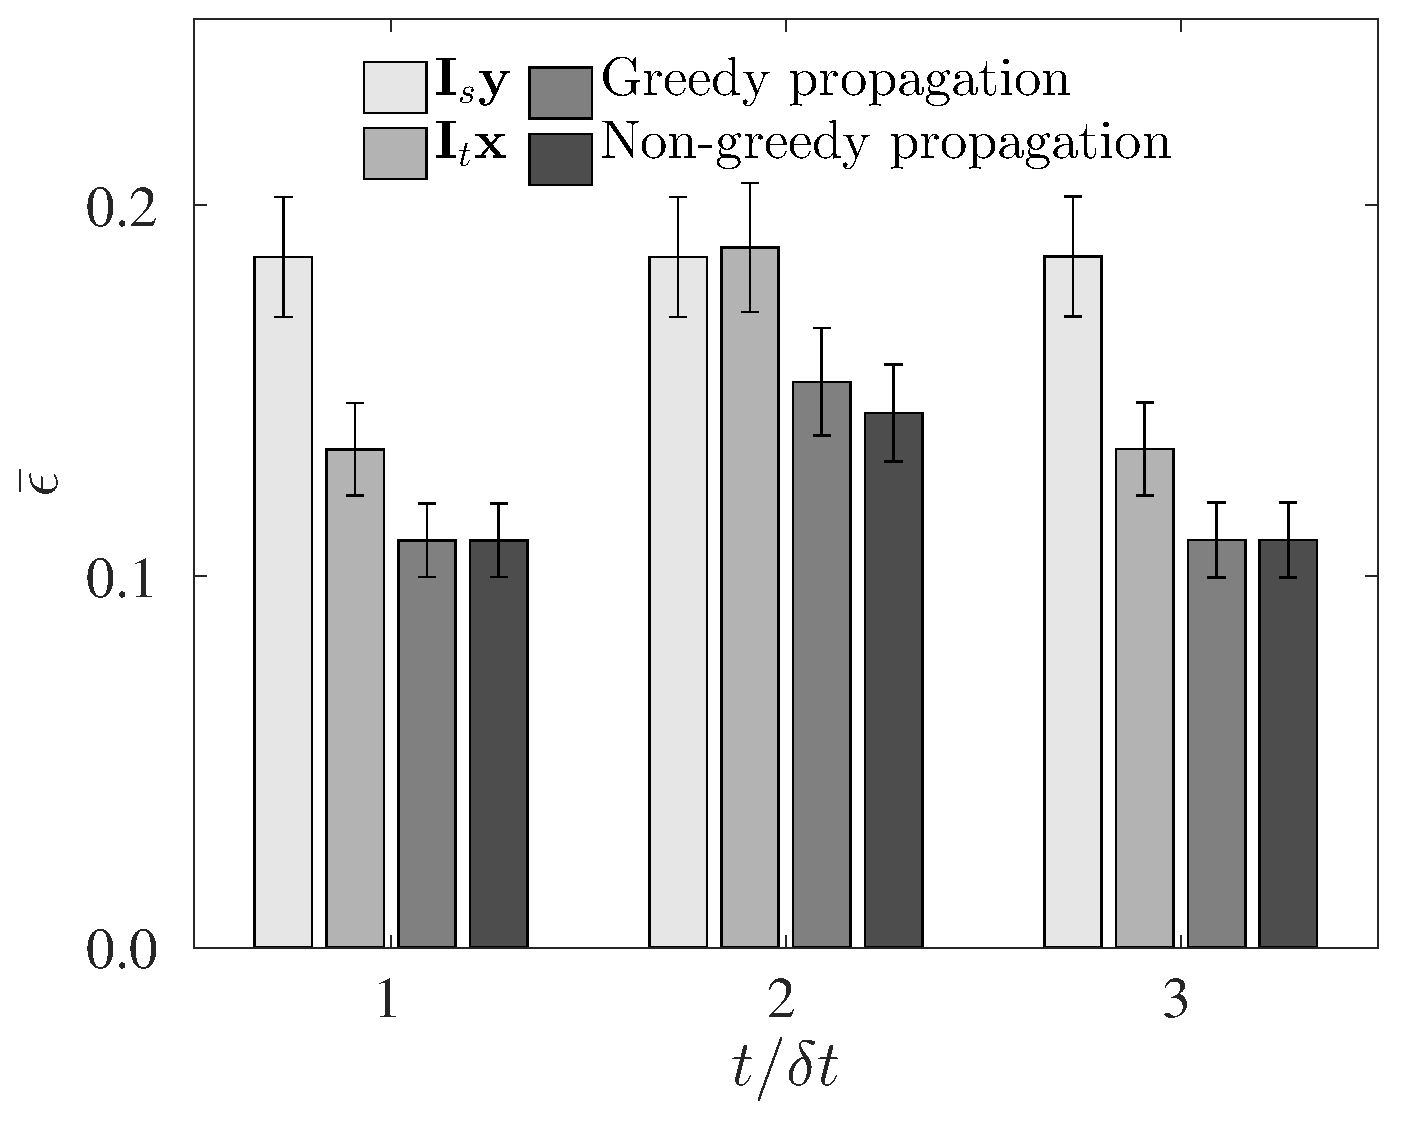
\includegraphics[width=.6\columnwidth]{./images/NLM/interpdiff/NLmean_interps_sspacing3_tspacing4_NRMSE.eps}
	\caption{\label{fig:NLmean_interps_sspacing3_tspacing4_NRMSE} Comparison of averaged NRMSEs as functions of time distances to the previous bounded LTHS plane by spatial/temporal interpolation, greedy and non-greedy propagation for the configuration where subsampling ratios are $ 3 \times 3 $ in space and $ 4 $ in time.}
\end{figure}

Figure \ref{fig:NLmean_interps_sspacing3_tspacing4_NRMSE} shows the mean NRMSEs by different methods as a function of time spacing to the previous LTHS plane $ t/\delta t $. The error bars are also shown, telling how these errors are different from one plane to another. These errors are estimated analogously as in figure \ref{fig:NLM_various_params_NRMSE}. NRMSEs of reconstructed fields obtained by propagation models or time interpolation are necessarily small close to the LTHS planes ($ t /\delta t = 1 $ and $ t /\delta t = 3 $), and increase toward the center. The error remains constant for spatial interpolation as it is only a function of the subsampling ratio in space. Greedy and non-greedy algorithms essentially give the same errors at the closest two planes from the LTHS ones. At these time steps, propagation models improve significantly (about $ 40 \% $) compared to spatial interpolation. At the middle plane, errors by propagation increase, but remain $ 20\% $ lower than both the interpolations. The non-greedy propagation model further decrease the error compared to the greedy one. 

\begin{figure}[t]
	\centering
	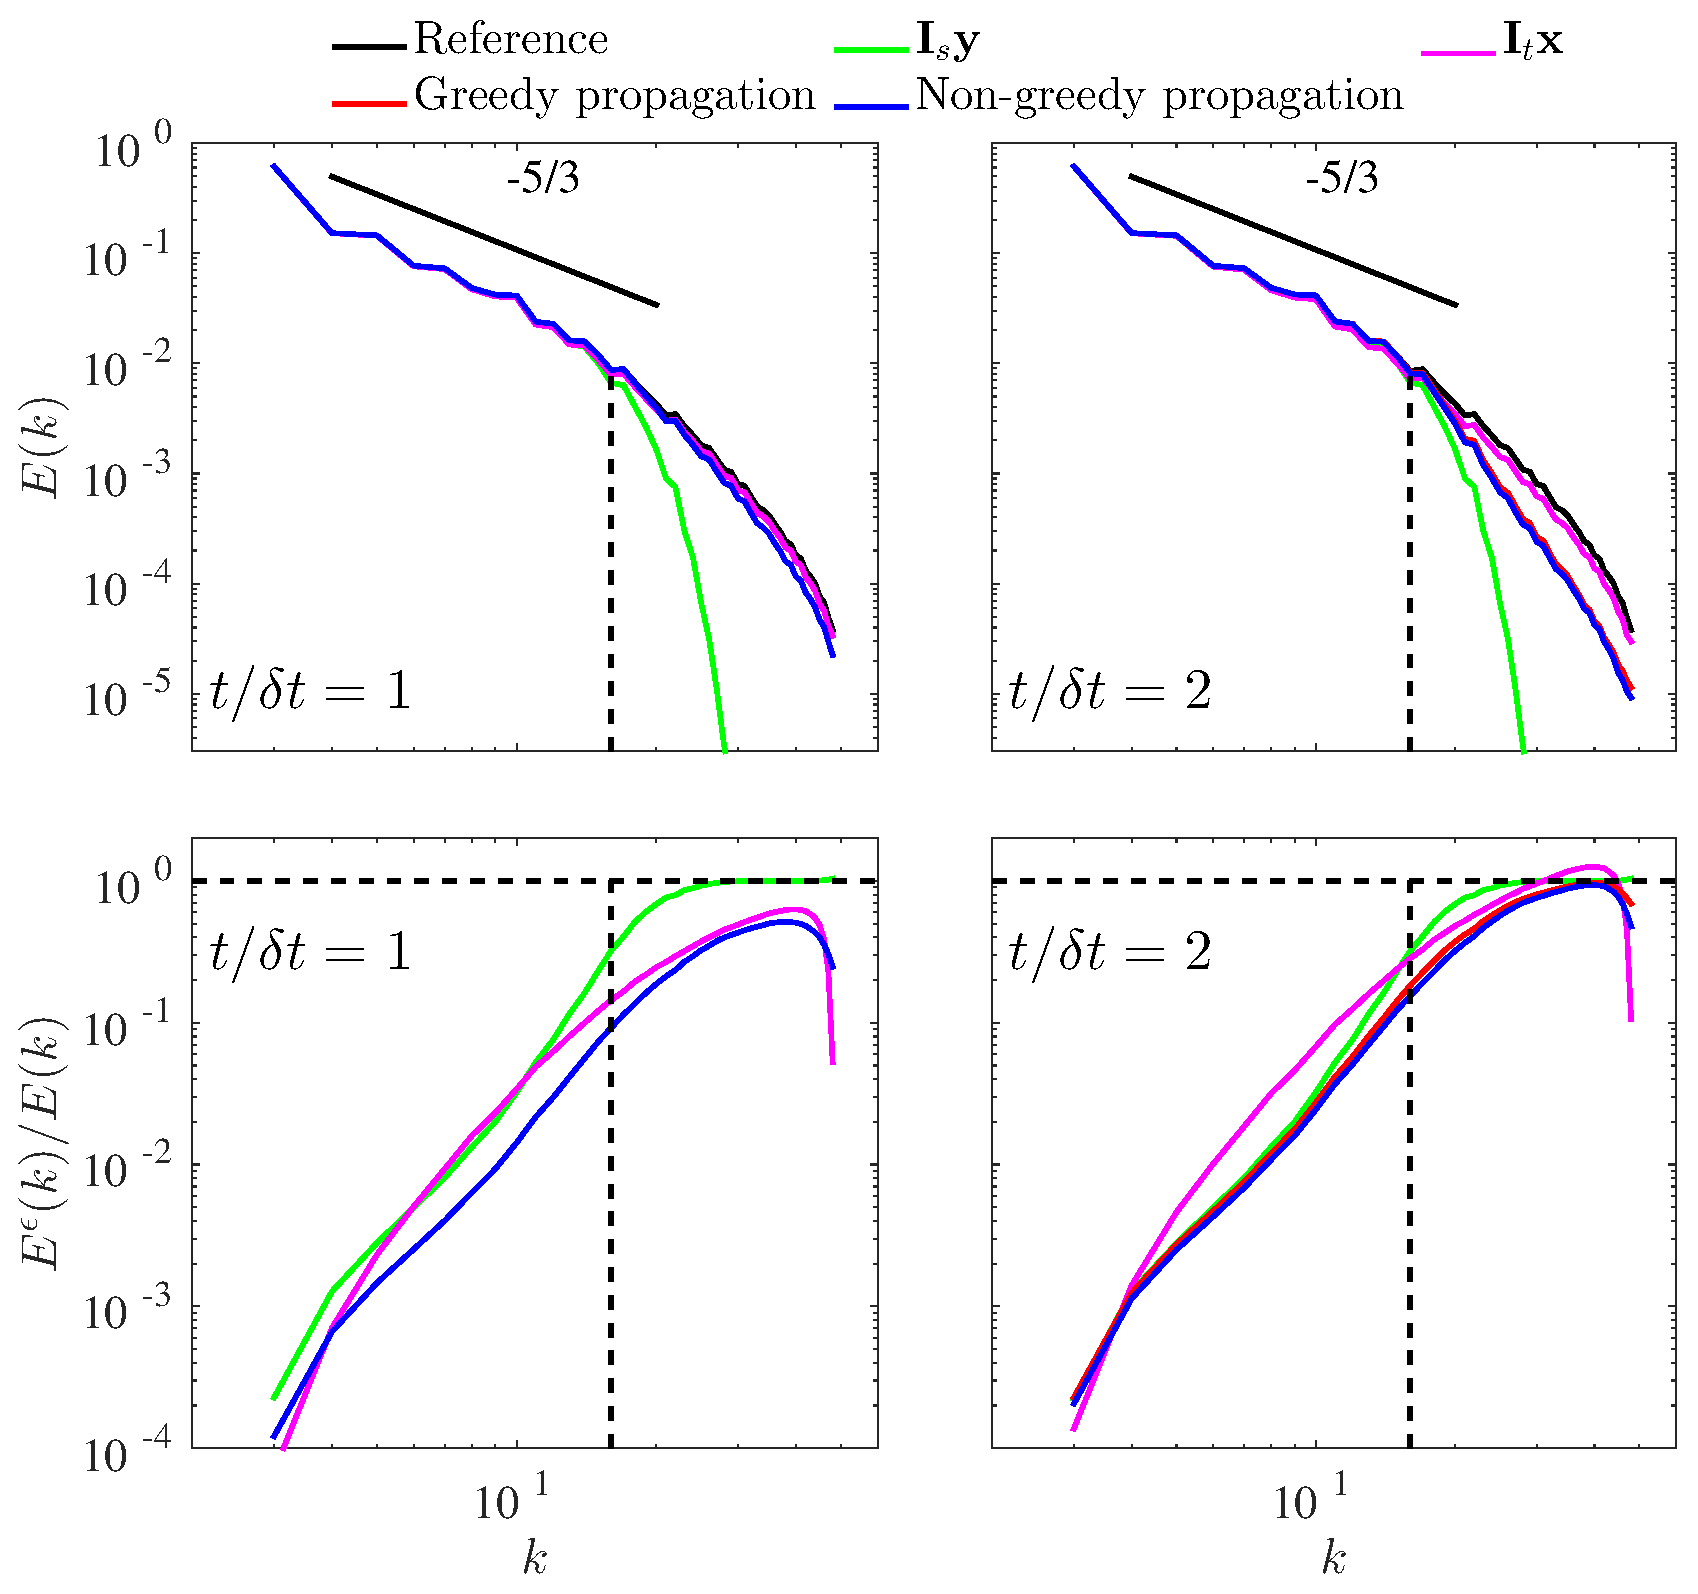
\includegraphics[width=\columnwidth]{./images/NLM/interpdiff/NLmean_interps_sspacing3_tspacing4_spectra2d.eps}		
	\caption{\label{fig:NLmean_interps_sspacing3_tspacing4_spectra2d} Comparison of energy spectra and error spectra for various reconstructions by spatial/temporal interpolation, greedy and non-greedy propagation. Subsampling ratios are $ 3 \times 3 $ in space and $ 4 $ in time. The spectra are averaged over all planes of the same distance to the closest LTHS plane, i.e. $ t/\delta t= 1 $ (left) or $t/\delta t= 2  $ (right).}
\end{figure}

Figure \ref{fig:NLmean_interps_sspacing3_tspacing4_spectra2d} shows the spectral analysis of the reconstruction by different models. Energy spectra and error spectra are shown for the two positions, either close or far from LTHS planes. From the first two spectra, it is shown that spatial interpolation captures only large-scale information. Time interpolation gives an estimate with a good energy spectrum, while propagation schemes are subject to a certain energy loss at small scales. However, the error spectra shows that time interpolation gives good energy spectra with poorly reconstructed small scales. Propagation models yield compromise estimates. Certain amount of small scales are captured, while error spectra illustrate improvements at all frequencies compared to both interpolations. 

\subsection{Model performances in various configurations}
\begin{table} 
	\caption{\label{tab:NLM_various_cases}
	Configuration parameters of six testing cases. The subsampling ratios of HTLS measurements are $ \sqrt{\dimsh/\dimsl} $ and equal in both spatial directions. The ratios of LTHS measurements in time are $ \dimth/\dimtl $. The normalized energy losses in space $\Delta\kappa_s$ and in time $\Delta\kappa_t$ are defined in Eq.~(\ref{eq:RMS_losses}).}
	\vspace{.5cm}
	\centering
	\begin{tabular}{ccS[table-format=1.0]S[table-format=1.0]cS[table-format=1.2]S[table-format=1.2]} 
		\toprule
		\multirow{2}{*}{Case}&\multicolumn{1}{c}{}&\multicolumn{2}{c}{Subsampling ratios}&\multicolumn{1}{c}{}&\multicolumn{2}{c}{Energy loss}\\ 
		\cmidrule{3-4} \cmidrule{6-7}
		 & & {$\sqrt{\dimsh/\dimsl}$} & $\dimth/\dimtl$ & & {$\Delta\kappa_s(\%)$} & {$\Delta\kappa_t (\%)$}\\ 
		\midrule 
		1 &  & 3  & 4 & & 1.03 & 1.23 \\ %\addlinespace
		2 &  & 3  & 6 & & 1.03 & 3.56 \\ %\addlinespace
		3 &  & 3  & 8 & & 1.03 & 6.53 \\ %\addlinespace
		4 &  & 3  & 4 & & 1.03 & 1.23 \\ %\addlinespace
		5 &  & 4  & 4 & & 2.63 & 1.23 \\ %\addlinespace	 
		6 &  & 6  & 4 & & 7.29 & 1.23 \\ %\addlinespace
		\bottomrule
	\end{tabular}
\end{table}

To characterize the proposed propagation models, various configurations at different subsampling ratios in either space or time are investigated. Model performances depend on the ratio in space, since it defines how much information is missing. The performances also depend on the ratio in time, since small-scale information will necessarily be lost when similarity between large scales die off with increasing time spacings. 

\begin{figure}[t]
	\centering
	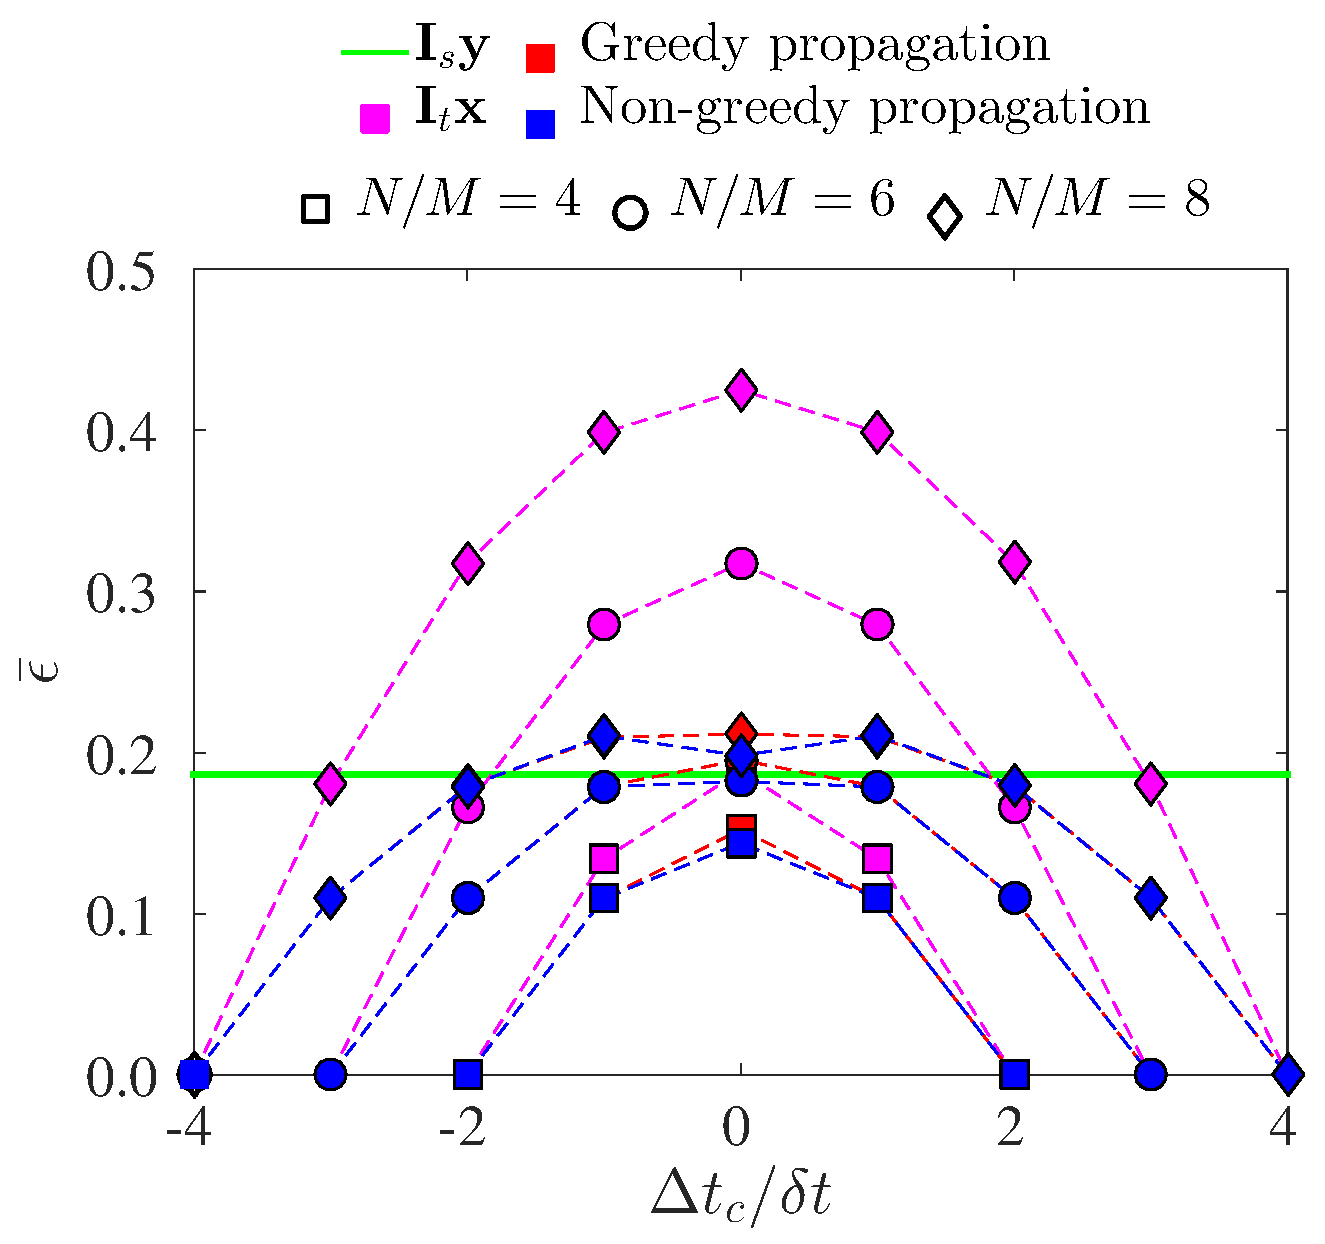
\includegraphics[width=0.65\columnwidth]{./images/NLM/interpdiff/NLmean_interps_NRMSE_vary_timespacing.eps}		
	\caption{\label{fig:NLmean_interps_NRMSE_vary_timespacing} Averaged NRMSEs of reconstruction by spatial/temporal interpolation, greedy and non-greedy propagation models. The errors are shown for three cases, with a fixed ratio in space $ (\dimsh/\dimsl = 3 \times 3) $ and varied ratios in time $(\dimth/\dimtl=4,6,8) $. The reference plane is chosen to be the mid-plane, and $ \Delta t_c/\delta t $ is the distance of each other plane from the reference one. Different colors refer to different methods, while the marker shapes vary for different $ \dimth/\dimtl $.}
\end{figure}

To test the model performances when increasing time distances between LTHS snapshots, the subsampling ratio $ \dimsh/\dimsl=3 \times 3 $ in space, while varying those in time as $ \dimth/\dimtl=4,6 $ and $ 8 $. The amount of missing information to recover due to the subsampling in space is about $ 1 \% $ of the total energy of the flow. Average NRMSEs as a function of the position in time are shown in figure \ref{fig:NLmean_interps_NRMSE_vary_timespacing}. In all three cases, the central plane is at $ \Delta t_c/\delta t = 0 $, while other planes are at different distances $ \Delta t_c/\delta t$ to this plane, both negative (planes before) or positive (plane after). 

In the figure \ref{fig:NLmean_interps_NRMSE_vary_timespacing}, NRMSE for spatial interpolation remains constant, since it is independent of time. Errors by time interpolations or propagation models increase when moving toward the center. For time interpolations, these errors increase dramatically when the time subsampling ratio is high. The proposed propagation models are able to bring down the errors compared to interpolation for small to moderate distances between LTHS planes. For very large ones ($ \dimth/\dimtl=8 $, diamond shape), the propagated small scales even slightly downgrade the given large-scale information from the spatial interpolation.

\begin{figure}[t]
	\centering
	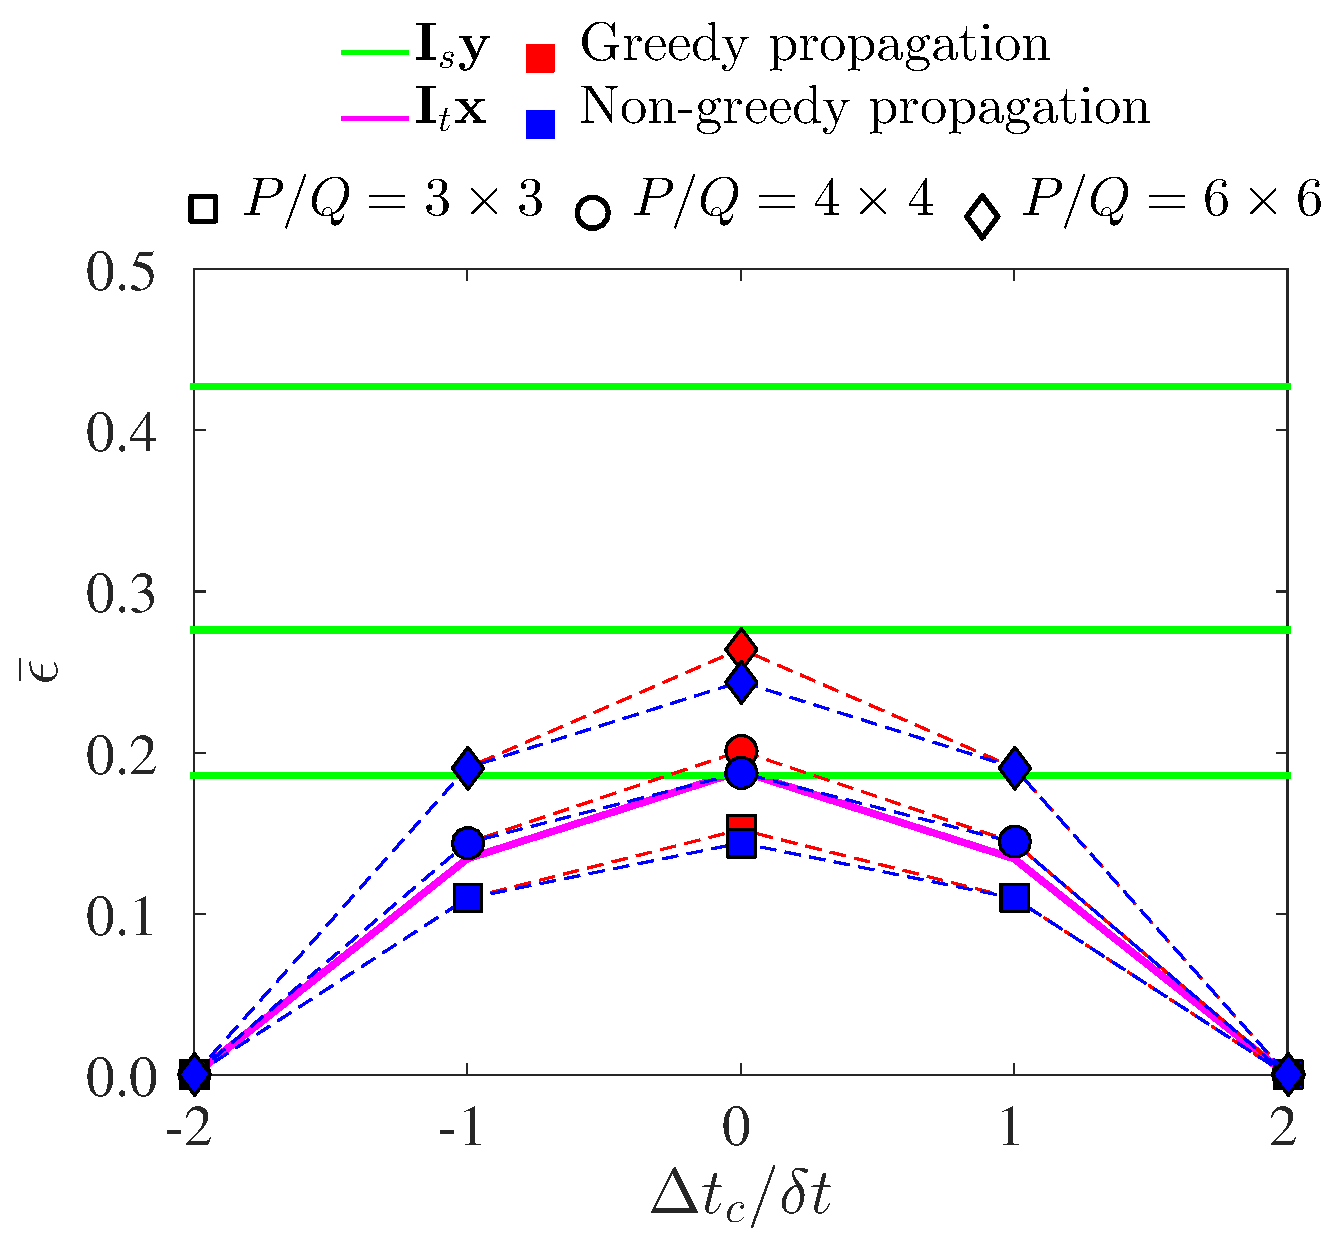
\includegraphics[width=0.65\columnwidth]{./images/NLM/interpdiff/NLmean_interps_NRMSE_vary_spacespacing.eps}		
	\caption{\label{fig:NLmean_interps_NRMSE_vary_spacespacing} Averaged NRMSEs of reconstruction by spatial/temporal interpolation, greedy and non-greedy propagation models. The errors are shown for different space spacing $ (\dimsh/\dimsl=3 \times , 4 \times 4, 6 \times 6) $, while in time the ratio is fixed $ (\dimth/\dimtl =4) $. The reference plane is chosen to be the mid-plane, and $ \Delta t_c/\delta t $ is the distance of each other plane from the reference one. Different colors refer to different methods, while the marker shapes vary for different $ \dimsh/\dimsl $.}
\end{figure}

Figure \ref{fig:NLmean_interps_NRMSE_vary_spacespacing} shows NRMSEs of the proposed propagation models (both greedy and non-greedy), spatial and temporal interpolations when varying the subsampling ratio in space as $ \dimsh/\dimsl = 3 \times 3, 4 \times 4 $ and $ 6 \times 6 $ while keeping a fixed distance between LTHS planes of $ \dimth/\dimtl=4 $. Time interpolation gives the same error for all three cases, while errors of spatial interpolations are independent of the position in time. For a small subsampling ratio in time, temporal interpolation and propagation models are always better than spatial interpolation. For a small ratio of $ \dimsh/\dimsl = 3 \times 3 $, the non-greedy propagation scheme give the most accurate reconstruction. In the case of moderate ratio ($ \dimsh/\dimsl=4 \times 4 $), the energy loss in space is already three times larger than that in time (see table \ref{tab:NLM_various_cases}). Propagation models start with large scales from spatial interpolation and reconstruct small-scale information to give the same accuracy as time interpolation. For a large subsampling ratio of $ \dimsh/\dimsl = 6 \times 6 $, propagation models improves significantly compared to spatial interpolation but remains worse than temporal interpolation. This is due to severe information losses after the subsampling in space, which cannot be  completely recovered.

\section{Concluding remarks}
The similarity-based propagation model, also called NLM-based propagation model, is proposed to reconstruct small scales in a configuration where measurements of all scales are given at key frames (LTHS planes). Small scales from these planes are propagated toward other instants in time. The proposed model takes benefits from the local/nonlocal similarity among scales and  among neighboring fields. Large-scale information is used as initial estimates and kept unchanged, while small scales are propagated as a weighted sum within a small neighborhood from one plane to another. The weights are estimated as the similarity of large scales in small patches. They are interpreted as the probabilities of an estimate to be its neighbors from nearby planes or key frames. 

The model works very well in the situation where the subsampling ratios are not severe. In such case, it is able to bring small scales of the flow and add to initial large scales given by the coarse measurements. It also performs better than temporal interpolation from key frames, which is point-wise and disregards the spatial structures of the flow. Among the models, the non-greedy propagation works the most accurately by gradually bringing small-scale information from the bounded planes toward the center. 

This model is not robust when the subsampling ratios remain moderate. When the time distance between LTHS planes increases, model performances are getting worse than spatial interpolation. This is because when the key frames are far from each other, similarities of large scales decay, making propagation models becomes inefficient. Reconstructed small-scale information even downgrades the initial large scales from spatial interpolation. The discrepancies are also found with large subsampling ratios in space. In such cases, the model suffers from severe information loss that can not be recovered completely. 

More sophisticated models can be further investigated to improve the reconstruction. First, it's worth mentioning the idea of multi-scale propagation, which has been investigated during this work but gives no improvement. However, in the case where the range of scales is extremely wide, there might be potential gain from a non-greedy propagation in space as the one in time presented in this chapter. Second, since structures in turbulence distort and rotate in a disorder manner, it maybe better to propose adapted methods that compute similarity of rotating patches. This idea has been started by \citet{zimmer2008rotationally}, but further investigation is required to adapt to our problem.


